\documentclass{article}
\usepackage[utf8]{inputenc}

\usepackage{latexsym}
\usepackage{float}
\usepackage[utf8]{inputenc}
%\usepackage[catalan]{babel}
 \usepackage[english]{babel}
\usepackage{microtype}
\usepackage[hyphens]{url}
\usepackage{hyperref}
\usepackage{graphicx}
\usepackage{makeidx}
\usepackage{datetime}
\usepackage{multicol}
\usepackage{setspace}
\usepackage{enumerate}
\usepackage{booktabs}
\usepackage{listings}
\usepackage{color}
\usepackage{amsmath}
\usepackage{amssymb}
\usepackage[table,xcdraw]{xcolor}
\usepackage{graphicx}
\usepackage{listings}
\usepackage{hyperref}
\usepackage{vmargin}
\usepackage{wrapfig}
\usepackage{subfiles}
\usepackage{float}
\usepackage{amsmath}
\usepackage{amssymb}
\usepackage{tikz-cd}
\usepackage{multirow}
\usepackage{pgffor}
\usepackage{iflang}
\usepackage{booktabs}
\usepackage{pgfplotstable}

%%%%%%%%%%%%%%%%%%%%%%%%%%%%%%%%%%%%%%%
%%%%%%%%%%%% UTIL COMMANDS %%%%%%%%%%%%  

\newcommand{\nc}{\newcommand}
\nc{\supindex}{\textsuperscript}

%%%%%%%%%%%%%%%%%%%%%%%%%%%%%%%%%%%%%%%
%%%%%%%%%%%%% CONFIG FILE %%%%%%%%%%%%%

\nc{\mytitle}{Preferential attachment}
\nc{\mysubtitle}{Report}
\nc{\authors}{Oriol Alàs Cercós, Sergi Simón Balcells}
\nc{\datetime}{28\supindex{th} of May, 2020}
\nc{\assignatura}{CiG}
\nc{\professorat}{Francesc Sebé}

% Per separar professors, utilitzar ','
% 	Ex: Maria, Joan, Pere

%%%%%%%%%%%%%%%%%%%%%%%%%%%%%%%%%%%%%%%
%%%%%%%%%%%%%  LANGUAGE   %%%%%%%%%%%%%

\newcommand{\tr}{\IfLanguageName{english}}

%%%%%%%%%%%%%%%%%%%%%%%%%%%%%%%%%%%%%%%
%%%%%%%%%%%%%%%%% MATH %%%%%%%%%%%%%%%%

\nc{\prob}[1]{P({#1})}
\nc{\probl}[2]{P({#1}|{#2})}

%%%%%%%%%%%%%%%%%%%%%%%%%%%%%%%%%%%%%%%
%%%%%%%%%%%%% TREE CREATOR %%%%%%%%%%%%

\setpapersize{A4}
\setmargins{2.5cm}  % margen izquierdo
{1.5cm}             % margen superior
{16.5cm}            % anchura del texto
{23.42cm}           % altura del texto
{10pt}              % altura de los encabezados
{1cm}               % espacio entre el texto y los encabezados
{0pt}               % altura del pie de página
{2cm}               % espaci\title{Determinització d'un autòmat finit}
\author{Oriol Alàs Cercós}
\date{29 d'Abril del 2019}

\def\contentsname{Índex}
\begin{document}
	

\begin{titlepage}
\begin{figure}[htb]
\begin{center}
	
\includegraphics[width=5cm]{imgs/UDL.png}
   	\vspace*{\stretch{1.0}}
   	\\
   	\medskip
   	\begin{center}
   		\noindent\rule{16.5cm}{0.4pt}
   		\medskip 
   		\\
      	\Huge\textbf{\mytitle}
      	\\\medskip 	\Large  \mysubtitle
      \\
      	
      	\noindent\rule{16.5cm}{0.4pt}
      	\\
      	\bigskip
      	\normalsize{\tr{Made by}{Realitzat per:}}
      	\\
      	\large\textit{\authors}
      	\\
      	\setlength{\parskip}{1em}
      	\normalsize{\tr{Delivery}{Data de lliurament:}}
      	\\
      	\large{\datetime}
   	\end{center}
   	\vspace*{\stretch{2.0}}
\end{center}
\end{figure}
\begin{flushright}
Universitat de Lleida
\\
Escola Politècnica Superior
\\
Grau en Enginyeria Informàtica
\\
\assignatura
\\
\medskip
\textbf{\tr{Professorate:}{Professorat:}}
\\
\foreach \n in \professorat{\n\\}
\end{flushright}
\thispagestyle{empty} 
\end{titlepage}
\tableofcontents
\thispagestyle{empty} 
%\newpage
\listoffigures
\listoftables
\thispagestyle{empty}
\newpage
\section{Introduction}
Using an anonymous and unlinkable ring signature-based forum, the way of choosing the K set of the signature ring can affect the privacy of users.
In this report is demonstrated that preferential attachment way makes users more anonymous and invulnerable from knowing its messages than uniformly random manner.
\subsection{Simulation program}
The simulation forum program was made in \texttt{python3}. The code can be found \href{https://github.com/sergisi/glowing-dollop}{here}. Its execution was made using 200 people and Zipf distribution to determine the number of messages of each member. Also, was parametrized the maximum number of messages from an author, in order to know which member can have the worst privacy. In all cases of s from 1.3 to 2.0, the number of messages determined from the distribution is 305.
\\
\\
The K, the size of the ring signature, ranges from 3 to 12. In order to compare the different ways of determining the signature, it is compared with authors of 1, 5 and 15 messages.\\
\\
The number of each table is calculated as an average of 10 random seeds for sampling 
the distribution. So, the meaning of $1$ message (msm) and $K=4$ and $s = 1.3$ means 
that on an average of $10$ times,  has a privacy score of $13.4$. The score of each element
is calculated by:
\[
			privacyScore(X) = 
			\frac
			{\# X\;\textrm{has signed a message}}
			{\# X\;\textrm{has really sended a message}}
\]
Given all the privacy scores of the different rings using a specific Zipf distribution, then is calculated the average of an specific member of them in order to compare, in general terms, the privacy between different Zipf distributions and different ring-signature methods.
\section{s: 1,3}
\begin{figure}[H] 
	\centering
	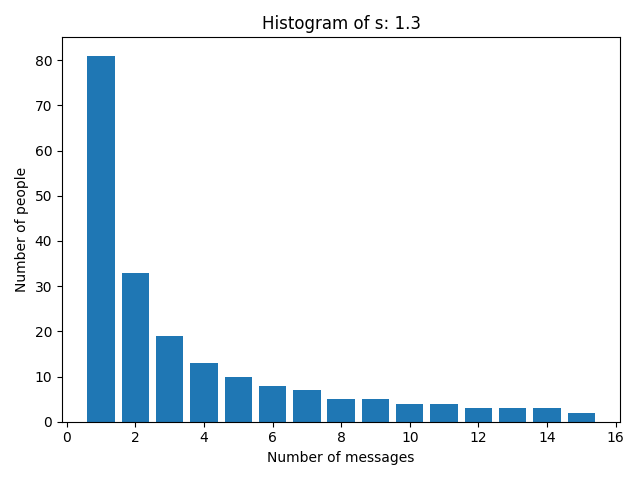
\includegraphics[width=10cm]{imgs/histogram-13.png}
	\caption{Histogram of Zipf Distribution using $s=1.3$}
	\label{fig:hist-13}
  \end{figure}
\begin{table}[H]
\centering
\begin{tabular}{c|ccc}
K &1msm &5msm &15msm\\
\hline
3 & 10.4 & 2.34 & 1.4533\\
4 & 13.4 & 2.86 & 1.7533\\
5 & 17.7 & 3.76 & 1.9533\\
6 & 21.4 & 4.34 & 2.2133\\
7 & 24.8 & 4.82 & 2.4933\\
8 & 28.7 & 5.62 & 2.72\\
9 & 32.5 & 6.36 & 2.9267\\
10 & 36.7 & 7.16 & 3.2533\\
11 & 40.8 & 7.96 & 3.3867\\
12 & 44.9 & 8.84 & 3.5467\\
\hline
& 27.13 & 5.406 & 2.57\\
\end{tabular}
\caption{Uniformly random choice of Zipf distribution s:1.3}
\label{tab:s1.3}
\end{table}

\begin{table}[H]
\centering
\begin{tabular}{c|ccc}
K &1msm &5msm &15msm\\
\hline
3 & 10.4 & 2.34 & 1.4533\\
4 & 13.4 & 2.86 & 1.7533\\
5 & 17.7 & 3.76 & 1.9533\\
6 & 21.4 & 4.34 & 2.2133\\
7 & 24.8 & 4.82 & 2.4933\\
8 & 28.7 & 5.62 & 2.72\\
9 & 32.5 & 6.36 & 2.9267\\
10 & 36.7 & 7.16 & 3.2533\\
11 & 40.8 & 7.96 & 3.3867\\
12 & 44.9 & 8.84 & 3.5467\\
\hline
& 27.13 & 5.406 & 2.57\\
\end{tabular}
\caption{Uniformly random choice of Zipf distribution s:1.3}
\label{tab:s1.3}
\end{table}

\section{s: 1,4}
\begin{figure}[H] \centering
 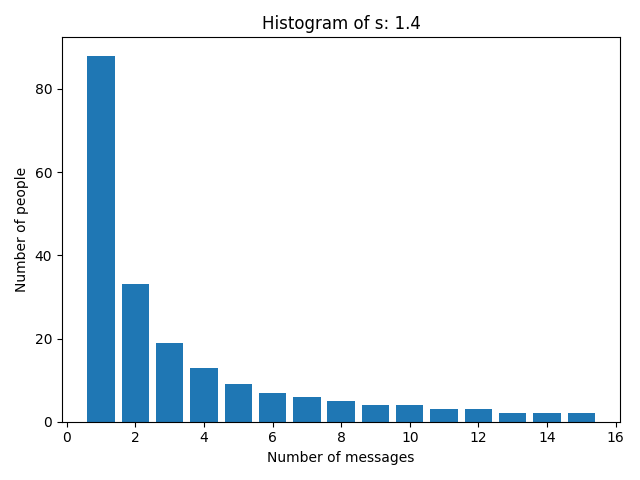
\includegraphics[width=10cm]{imgs/histogram-14.png}
 \label{fig:hist-14}
 \caption{Histogram of Zipf Distribution using $s=1.4$} \end{figure}

	\begin{table}[H]
		\begin{tabular}{c|ccc}
			\multicolumn{4}{c}{S:1.4}\\\hline
			3 & 10.6 & 2.12 & 2.24\\
			4 & 17.7 & 3.48 & 2.4\\
			5 & 25.6 & 3.66 & 2.8733\\
			6 & 33.0 & 4.3 & 2.88\\
			7 & 38.1 & 5.66 & 3.4667\\
			8 & 45.1 & 6.1 & 3.28\\
			9 & 46.5 & 7.18 & 4.1267\\
			10 & 53.2 & 8.6 & 3.88\\
			11 & 56.6 & 8.32 & 4.28\\
			12 & 72.8 & 7.26 & 3.58\\
			\hline
			& 39.92 & 5.668 & 3.3007\\
		\end{tabular}
	\end{table}

	\begin{table}[H]
		\begin{tabular}{c|ccc}
			\multicolumn{4}{c}{S:1.4}\\\hline
			3 & 10.6 & 2.12 & 2.24\\
			4 & 17.7 & 3.48 & 2.4\\
			5 & 25.6 & 3.66 & 2.8733\\
			6 & 33.0 & 4.3 & 2.88\\
			7 & 38.1 & 5.66 & 3.4667\\
			8 & 45.1 & 6.1 & 3.28\\
			9 & 46.5 & 7.18 & 4.1267\\
			10 & 53.2 & 8.6 & 3.88\\
			11 & 56.6 & 8.32 & 4.28\\
			12 & 72.8 & 7.26 & 3.58\\
			\hline
			& 39.92 & 5.668 & 3.3007\\
		\end{tabular}
	\end{table}


\section{s: 1,5}
\begin{figure}[H] \centering
 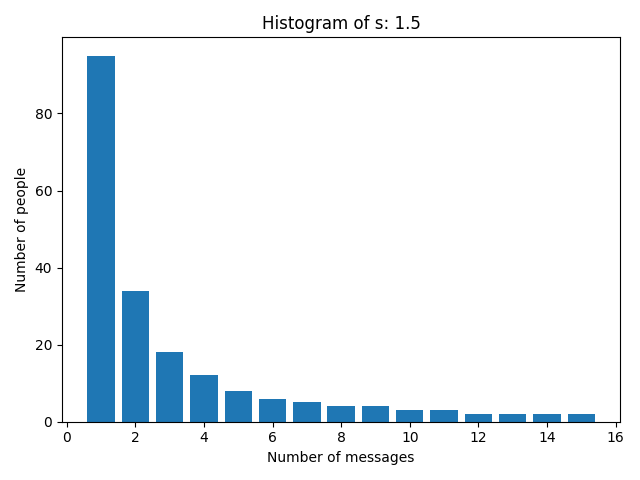
\includegraphics[width=10cm]{imgs/histogram-15.png}
 \label{fig:hist-15}
 \caption{Histogram of Zipf Distribution using $s=1.5$} \end{figure}
\begin{table}[H]
\centering
\begin{tabular}{c|ccc}
K &1msm &5msm &15msm\\
\hline
3 & 8.9 & 2.12 & 1.3933\\
4 & 12.2 & 2.5 & 1.62\\
5 & 16.0 & 3.16 & 1.7733\\
6 & 18.6 & 3.9 & 2.0733\\
7 & 22.2 & 4.58 & 2.1867\\
8 & 25.3 & 4.98 & 2.38\\
9 & 30.0 & 5.66 & 2.5867\\
10 & 31.9 & 6.36 & 2.88\\
11 & 34.9 & 7.02 & 3.0333\\
12 & 39.4 & 7.14 & 3.2867\\
\hline
& 23.94 & 4.742 & 2.3213\\
\end{tabular}
\caption{Simulation method:uniform simulation S:1.5}
\label{tab:s1.5}
\end{table}

\begin{table}[H]
\centering
\begin{tabular}{c|ccc}
K &1msm &5msm &15msm\\
\hline
3 & 8.9 & 2.12 & 1.3933\\
4 & 12.2 & 2.5 & 1.62\\
5 & 16.0 & 3.16 & 1.7733\\
6 & 18.6 & 3.9 & 2.0733\\
7 & 22.2 & 4.58 & 2.1867\\
8 & 25.3 & 4.98 & 2.38\\
9 & 30.0 & 5.66 & 2.5867\\
10 & 31.9 & 6.36 & 2.88\\
11 & 34.9 & 7.02 & 3.0333\\
12 & 39.4 & 7.14 & 3.2867\\
\hline
& 23.94 & 4.742 & 2.3213\\
\end{tabular}
\caption{Simulation method:uniform simulation S:1.5}
\label{tab:s1.5}
\end{table}



\section{s: 1,6}

\begin{figure}[H] \centering
 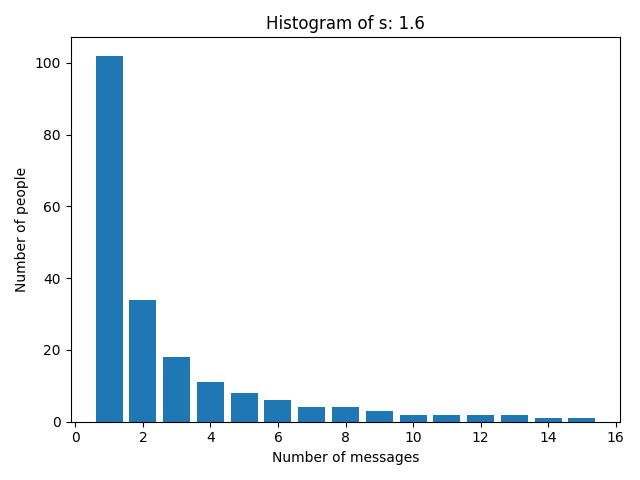
\includegraphics[width=10cm]{imgs/histogram-16.png}
 \label{fig:hist-16}
 \caption{Histogram of Zipf Distribution using $s=1.6$} \end{figure}
\begin{table}[H]
\centering
\begin{tabular}{c|ccc}
K &1msm &5msm &15msm\\
\hline
3 & 8.3 & 2.22 & 1.3067\\
4 & 11.4 & 2.94 & 1.5667\\
5 & 15.3 & 3.28 & 1.7\\
6 & 17.8 & 3.92 & 1.9133\\
7 & 20.1 & 4.56 & 2.0333\\
8 & 23.0 & 5.1 & 2.24\\
9 & 27.3 & 5.44 & 2.4667\\
10 & 29.8 & 6.12 & 2.52\\
11 & 31.6 & 6.68 & 2.7133\\
12 & 35.0 & 7.18 & 2.9267\\
\hline
& 21.96 & 4.744 & 2.1387\\
\end{tabular}
\caption{Uniformly random choice of Zipf distribution s:1.6}
\label{tab:s1.6}
\end{table}

\begin{table}[H]
\centering
\begin{tabular}{c|ccc}
K &1msm &5msm &15msm\\
\hline
3 & 8.3 & 2.22 & 1.3067\\
4 & 11.4 & 2.94 & 1.5667\\
5 & 15.3 & 3.28 & 1.7\\
6 & 17.8 & 3.92 & 1.9133\\
7 & 20.1 & 4.56 & 2.0333\\
8 & 23.0 & 5.1 & 2.24\\
9 & 27.3 & 5.44 & 2.4667\\
10 & 29.8 & 6.12 & 2.52\\
11 & 31.6 & 6.68 & 2.7133\\
12 & 35.0 & 7.18 & 2.9267\\
\hline
& 21.96 & 4.744 & 2.1387\\
\end{tabular}
\caption{Uniformly random choice of Zipf distribution s:1.6}
\label{tab:s1.6}
\end{table}



\section{s: 1,7}

\begin{figure}[H] \centering
 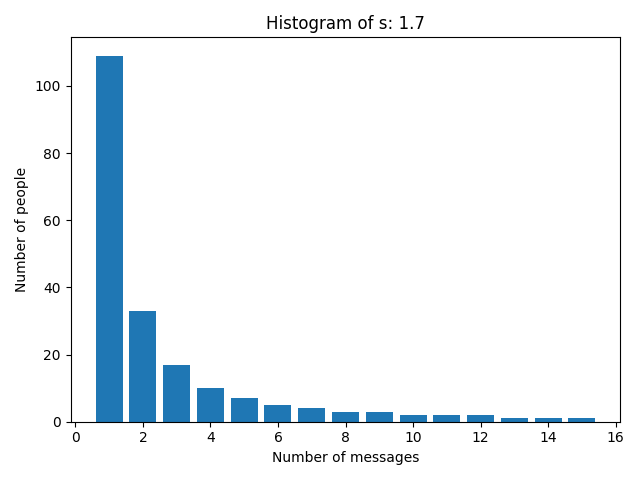
\includegraphics[width=10cm]{imgs/histogram-17.png}
 \label{fig:hist-17}
 \caption{Histogram of Zipf Distribution using $s=1.7$} \end{figure}
\begin{table}[H]
\centering
\begin{tabular}{c|ccc}
K &1msm &5msm &15msm\\
\hline
3 & 9.6 & 1.9 & 1.78\\
4 & 13.3 & 2.96 & 2.2733\\
5 & 18.1 & 3.58 & 2.52\\
6 & 22.3 & 3.62 & 2.7933\\
7 & 26.4 & 4.26 & 2.8867\\
8 & 32.7 & 4.76 & 3.2333\\
9 & 36.0 & 6.52 & 4.08\\
10 & 41.0 & 5.18 & 3.8133\\
11 & 43.6 & 7.5 & 4.02\\
12 & 47.6 & 6.32 & 3.34\\
\hline
& 29.06 & 4.66 & 3.074\\
\end{tabular}
\caption{S:1.7}
\label{tab:s1.7}
\end{table}

\begin{table}[H]
\centering
\begin{tabular}{c|ccc}
K &1msm &5msm &15msm\\
\hline
3 & 9.6 & 1.9 & 1.78\\
4 & 13.3 & 2.96 & 2.2733\\
5 & 18.1 & 3.58 & 2.52\\
6 & 22.3 & 3.62 & 2.7933\\
7 & 26.4 & 4.26 & 2.8867\\
8 & 32.7 & 4.76 & 3.2333\\
9 & 36.0 & 6.52 & 4.08\\
10 & 41.0 & 5.18 & 3.8133\\
11 & 43.6 & 7.5 & 4.02\\
12 & 47.6 & 6.32 & 3.34\\
\hline
& 29.06 & 4.66 & 3.074\\
\end{tabular}
\caption{S:1.7}
\label{tab:s1.7}
\end{table}



\section{s: 1,8}

\begin{figure}[H] \centering
 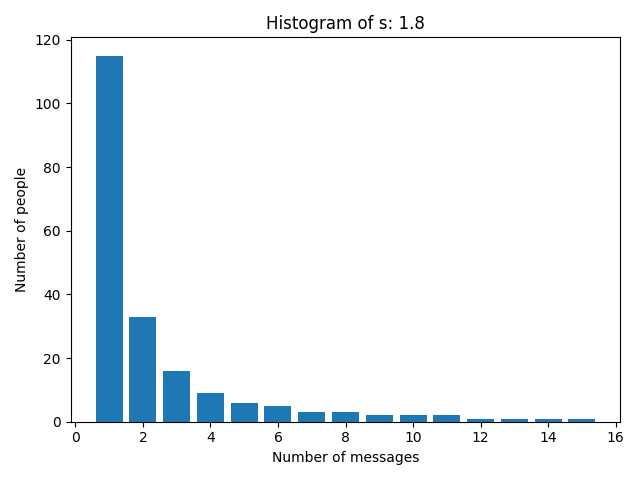
\includegraphics[width=10cm]{imgs/histogram-18.png}
 \label{fig:hist-18}
 \caption{Histogram of Zipf Distribution using $s=1.8$} \end{figure}
\begin{table}[H]
\centering
\begin{tabular}{c|ccc}
K &1msm &5msm &15msm\\
\hline
3 & 7.3 & 2.68 & 1.8667\\
4 & 10.9 & 3.54 & 2.2933\\
5 & 15.1 & 2.9 & 2.2267\\
6 & 19.8 & 3.96 & 2.9067\\
7 & 23.9 & 3.04 & 2.96\\
8 & 27.8 & 4.16 & 3.6733\\
9 & 32.5 & 4.22 & 4.36\\
10 & 35.9 & 5.3 & 3.6267\\
11 & 35.3 & 4.56 & 3.8267\\
12 & 42.2 & 5.44 & 3.8733\\
\hline
& 25.07 & 3.98 & 3.1613\\
\end{tabular}
\caption{S:1.8}
\label{tab:s1.8}
\end{table}

\begin{table}[H]
\centering
\begin{tabular}{c|ccc}
K &1msm &5msm &15msm\\
\hline
3 & 7.3 & 2.68 & 1.8667\\
4 & 10.9 & 3.54 & 2.2933\\
5 & 15.1 & 2.9 & 2.2267\\
6 & 19.8 & 3.96 & 2.9067\\
7 & 23.9 & 3.04 & 2.96\\
8 & 27.8 & 4.16 & 3.6733\\
9 & 32.5 & 4.22 & 4.36\\
10 & 35.9 & 5.3 & 3.6267\\
11 & 35.3 & 4.56 & 3.8267\\
12 & 42.2 & 5.44 & 3.8733\\
\hline
& 25.07 & 3.98 & 3.1613\\
\end{tabular}
\caption{S:1.8}
\label{tab:s1.8}
\end{table}



\section{s: 1,9}

\begin{figure}[H] \centering
 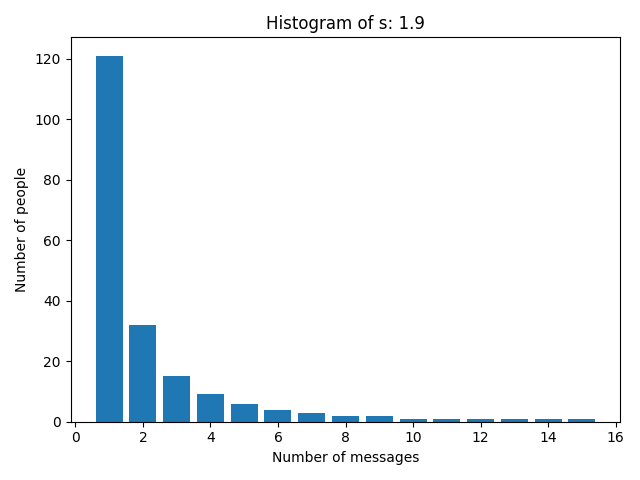
\includegraphics[width=10cm]{imgs/histogram-19.png}
 \label{fig:hist-19}
 \caption{Histogram of Zipf Distribution using $s=1.9$} \end{figure}
\begin{table}[H]
\centering
\begin{tabular}{c|ccc}
K &1msm &5msm &15msm\\
\hline
3 & 6.0 & 1.72 & 1.2533\\
4 & 9.5 & 2.22 & 1.42\\
5 & 13.5 & 2.52 & 1.6\\
6 & 15.3 & 2.8 & 1.7933\\
7 & 17.9 & 3.28 & 1.8333\\
8 & 19.7 & 3.64 & 1.9933\\
9 & 22.1 & 3.82 & 2.1533\\
10 & 24.4 & 4.46 & 2.26\\
11 & 26.5 & 4.82 & 2.48\\
12 & 30.0 & 5.48 & 2.6\\
\hline
& 18.49 & 3.476 & 1.9387\\
\end{tabular}
\caption{Uniformly random choice of Zipf distribution s:1.9}
\label{tab:s1.9}
\end{table}

\begin{table}[H]
\centering
\begin{tabular}{c|ccc}
K &1msm &5msm &15msm\\
\hline
3 & 6.0 & 1.72 & 1.2533\\
4 & 9.5 & 2.22 & 1.42\\
5 & 13.5 & 2.52 & 1.6\\
6 & 15.3 & 2.8 & 1.7933\\
7 & 17.9 & 3.28 & 1.8333\\
8 & 19.7 & 3.64 & 1.9933\\
9 & 22.1 & 3.82 & 2.1533\\
10 & 24.4 & 4.46 & 2.26\\
11 & 26.5 & 4.82 & 2.48\\
12 & 30.0 & 5.48 & 2.6\\
\hline
& 18.49 & 3.476 & 1.9387\\
\end{tabular}
\caption{Uniformly random choice of Zipf distribution s:1.9}
\label{tab:s1.9}
\end{table}



\section{s: 2,0}

\begin{figure}[H] \centering
 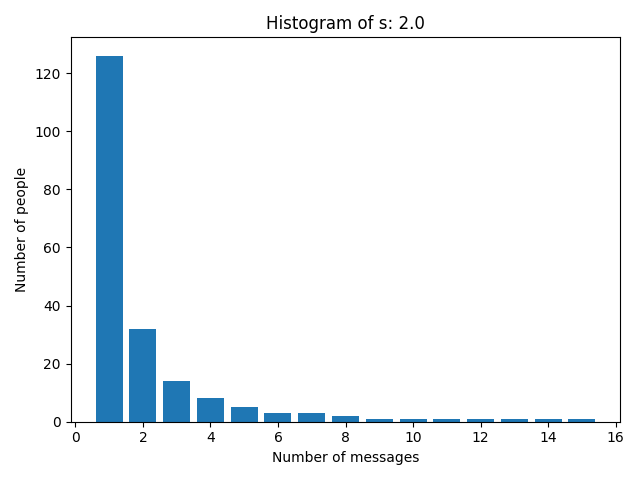
\includegraphics[width=10cm]{imgs/histogram-20.png}
 \label{fig:hist-20}
 \caption{Histogram of Zipf Distribution using $s=2.0$} \end{figure}
\begin{table}[H]
\centering
\begin{tabular}{c|ccc}
K &1msm &5msm &15msm\\
\hline
3 & 6.5 & 2.62 & 1.66\\
4 & 9.5 & 3.1 & 2.1533\\
5 & 14.2 & 3.84 & 2.3933\\
6 & 17.5 & 4.42 & 2.74\\
7 & 20.7 & 5.42 & 2.7733\\
8 & 23.6 & 3.58 & 3.14\\
9 & 26.8 & 6.34 & 3.7667\\
10 & 29.2 & 4.94 & 3.14\\
11 & 32.0 & 5.5 & 3.7133\\
12 & 36.0 & 7.9 & 4.4933\\
\hline
& 21.6 & 4.766 & 2.9973\\
\end{tabular}
\caption{S:2.0}
\label{tab:s2.0}
\end{table}

\begin{table}[H]
\centering
\begin{tabular}{c|ccc}
K &1msm &5msm &15msm\\
\hline
3 & 6.5 & 2.62 & 1.66\\
4 & 9.5 & 3.1 & 2.1533\\
5 & 14.2 & 3.84 & 2.3933\\
6 & 17.5 & 4.42 & 2.74\\
7 & 20.7 & 5.42 & 2.7733\\
8 & 23.6 & 3.58 & 3.14\\
9 & 26.8 & 6.34 & 3.7667\\
10 & 29.2 & 4.94 & 3.14\\
11 & 32.0 & 5.5 & 3.7133\\
12 & 36.0 & 7.9 & 4.4933\\
\hline
& 21.6 & 4.766 & 2.9973\\
\end{tabular}
\caption{S:2.0}
\label{tab:s2.0}
\end{table}

\end{document}
